% -*- mode: latex; mode: auto-fill; coding: utf-8; -*-

\chapter{Conclusion}

We have created an exciting dynamic outdoor environment that changes
look and feel according the time of day. To do this we have used
OpenGL's programmable pipeline and some of OpenGL new extensions.

The time of day is easy to see when looking at the sky. At day time
the sky is bright blue with animated clouds, at night star fields fill
the sky, and at sunrise and sunset yellow and red scattered sunlight
can be seen along the horizon.
%
Details have been added to the terrain by using advanced lighting
techniques, such as bump mapping, and waving grass makes it come alive.
%
A final level of detail is provided by the our new post processing
extension which includes effects such as motion blur, glow, and depth of
field. Other effects such as edge detection and an underwater post
processing effect have already been created and applied to other
OpenEngine projects, so we also succeeded in creating an easy-to-use
interface, which will hopefully be of use to many.

All in all, we are quite satisfied with the look and feel of the end
result.


%Post Process

%% Storing and rebinding the previous framebuffer means that we can chain
%% several post process nodes together to form complex effects or
%% minimize the cost of applying an effect by using for example separable
%% convolution.

% One/two fbos pr node is a waste but makes it easy to setup and they
% can be configured individually

% Other effects have been implemented, like wobble, edge detection,
% pixelate and an underwater that combines...



\section{Future work}

Although we have come a long way there are still things that we wish
to do even better. The following techniques have been discussed during
the development of the project.

The current terrain implementation could be replaced by a clipmap
implementation. Level of detail should also be extended to not only
apply to textures and geometry, but also the shaders. An example would
be removing specular lighting and bumpmapping from shaders on distant
terrain. An alternative to the current geomorphing LOD system is
alpha blending, which would make transitions between LODs not require
that morphing is handled, but of course means we'd have to handle
transparency instead.

Our sky implementation currently have two minor visual defects: The
first problem is that the atmospheric dome do not take the angle of
the sun into account. This results in a uniform coloring of the dome
in the vertical direction on the entire sphere. A more realistic
coloring would be to only color the dome shades of yellow and red in a
radius around where the sun is setting or rising.
%
We have also talked about going even further an implementing a full
atmospheric scattering simulation algorithm like the
effect described in \citebook{chapter~16}{GPUGEMS2}.
%
The second problem is that the texture mapping of the cloud dome does
not have the right perspective.
To fixed this we have talked about using the texture mapping scheme
based on a plane as described in \citebook{page~32}{copenhagen2007real}.

When generating the cloud texture we use value noise as suggested in
the web page that inspired our
work\footnote{\url{http://freespace.virgin.net/hugo.elias/models/m_perlin.htm}}.
Some authors however use Perlin noise to generate clouds, which could
be interesting to implement and compare with our current value noise.

The next step for the \class{PostProcessNode} is to allow it to be
placed anywhere inside the scene graph and then merge the post
processed image with the rest of the scene. An optimized versions of
some of the most commonly used effects could also be made to increase
performance and in the case of Depth of Field remove the flickering
that comes from only sampling one focus point.

During our work with texture binding the idea of creating a texture
binding manager that reuses \emph{texture unit} using
\code{glActivateTexture}\citebook{page~440}{redbook} has
surfaced. This manager could cache texture ids and texture units so
the last x number of bound textures more quickly can be activated.

\begin{figure}
  \centering
  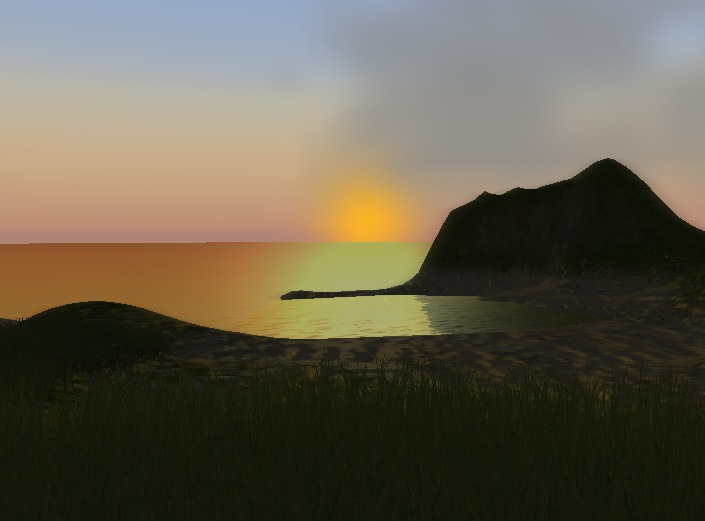
\includegraphics[width=12cm]{sunset}
\end{figure}
